\documentclass[12pt]{article}
\usepackage{packages}

\begin{document}
\section*{Exercise 1}

\subsection*{(a)}
\begin{figure}[h]
\centering
\begin{minipage}{0.47\textwidth}
    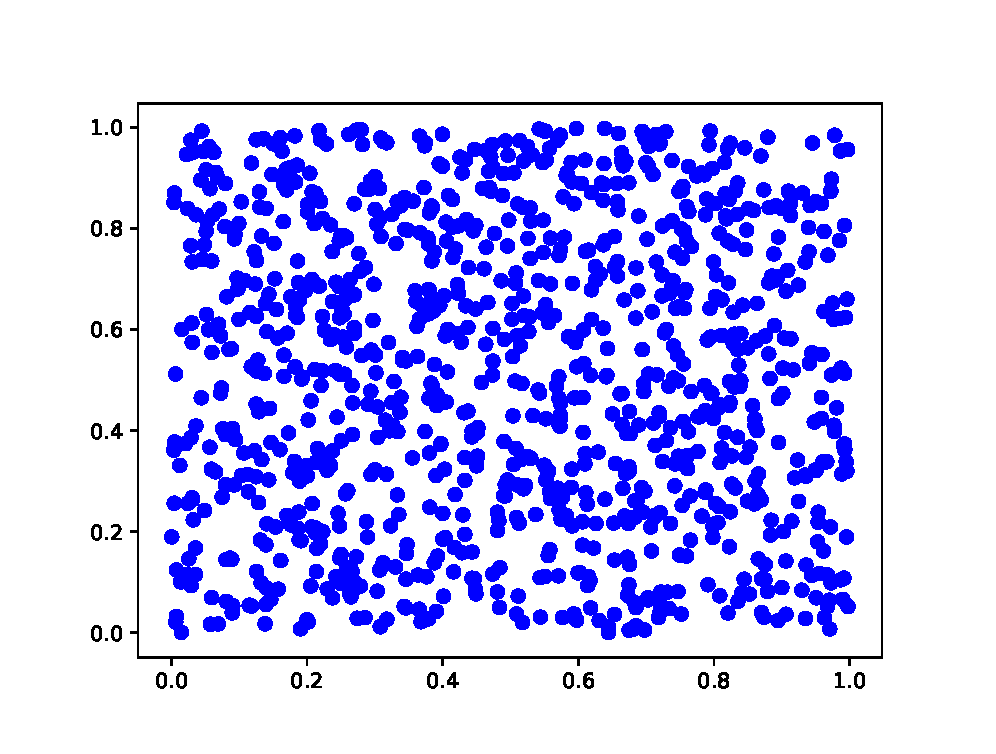
\includegraphics[width=1.2\textwidth]{figures/mt19937.eps}
    \captionof{figure}{mt19937}
\end{minipage}
\hfill
\begin{minipage}{0.47\textwidth}
    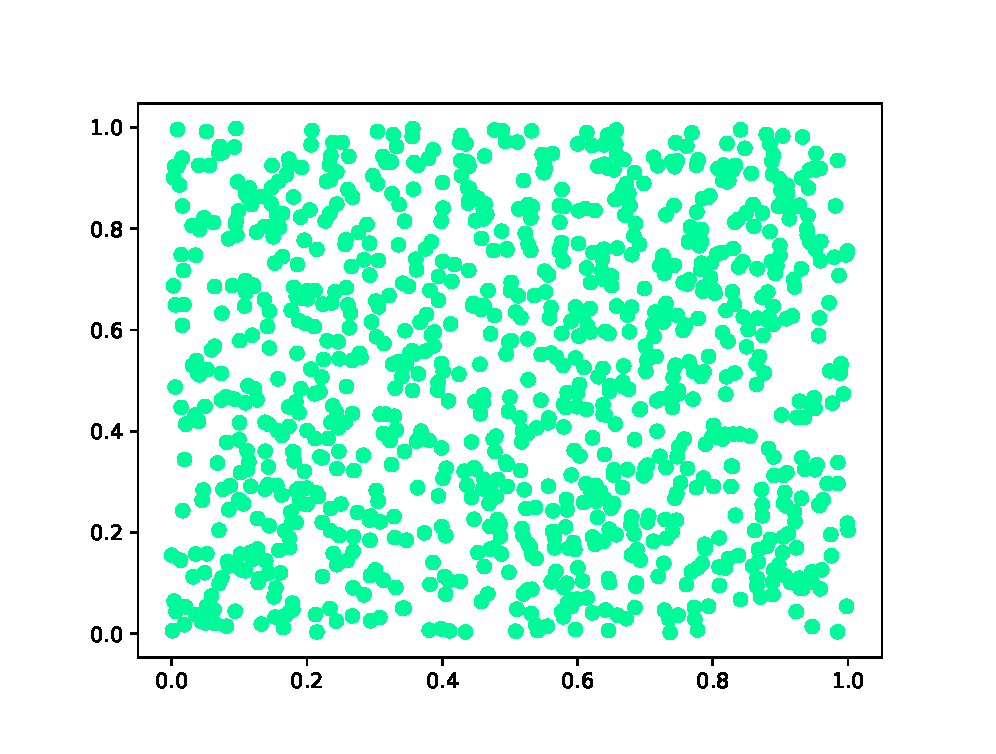
\includegraphics[width=1.2\textwidth]{figures/builtin.eps}
    \captionof{figure}{c++ rand()}
\end{minipage}
\end{figure}
\begin{figure}[h]
    \centering
    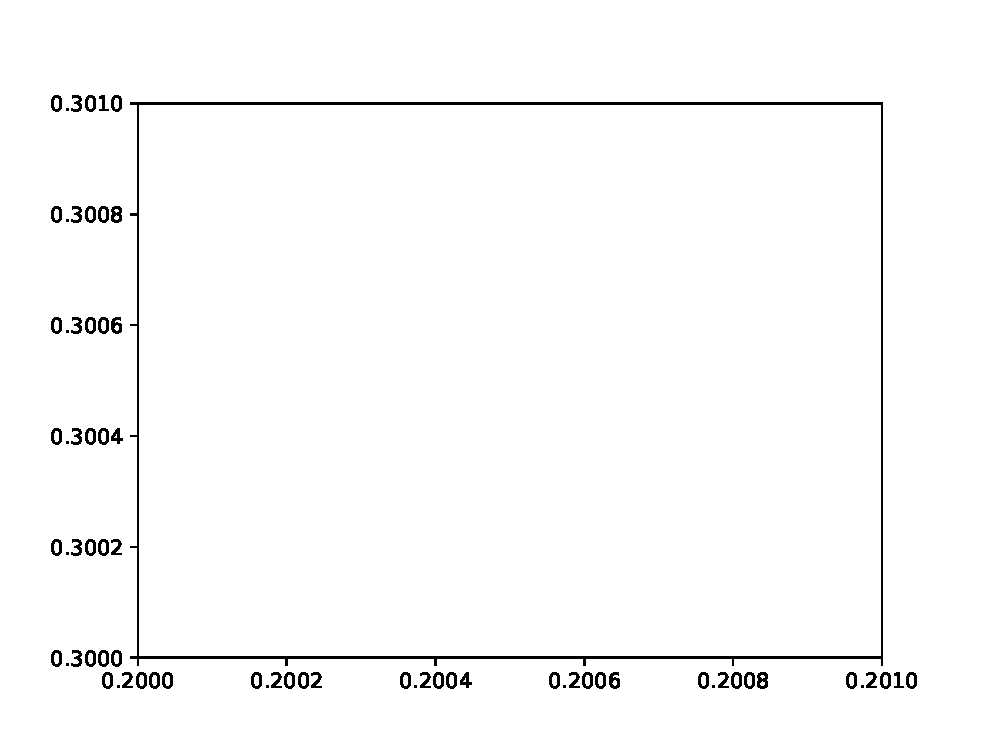
\includegraphics[width=0.7\textwidth]{figures/randu.eps}
    \captionof{figure}{RANDU}
\end{figure}

\newpage

\subsection*{(b)}

\begin{figure}[h]
    \centering
    \begin{minipage}{0.47\textwidth}
        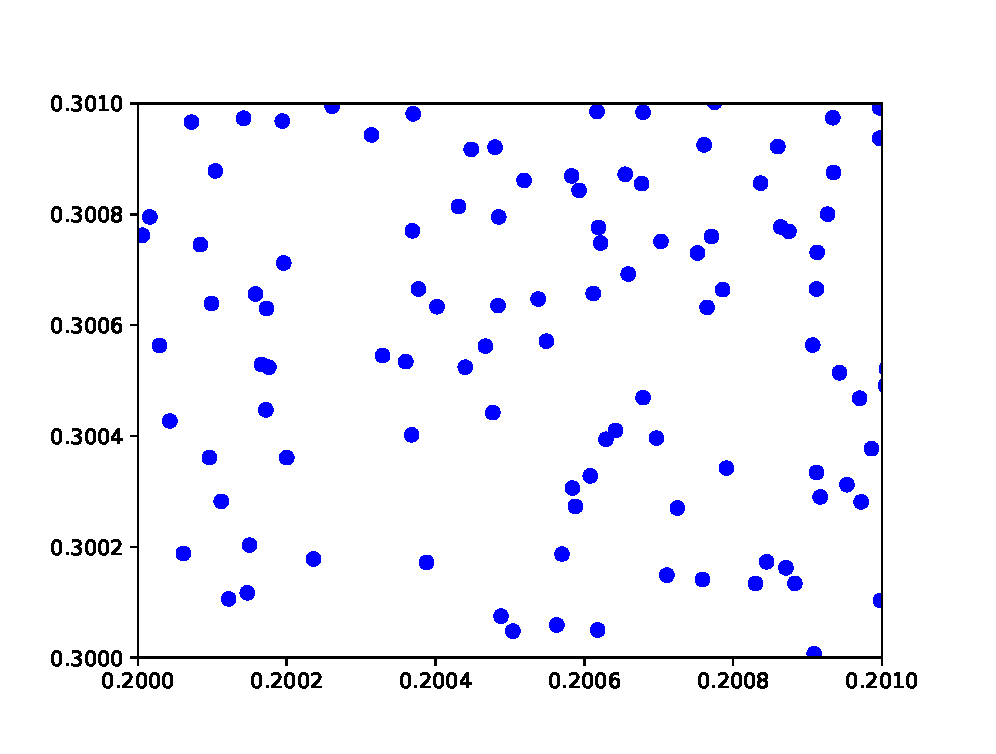
\includegraphics[width=1.2\textwidth]{figures/mt19937_zoomed.eps}
        \caption{mt19937 zoomed}
    \end{minipage}
    \hfill
    \begin{minipage}{0.47\textwidth}
        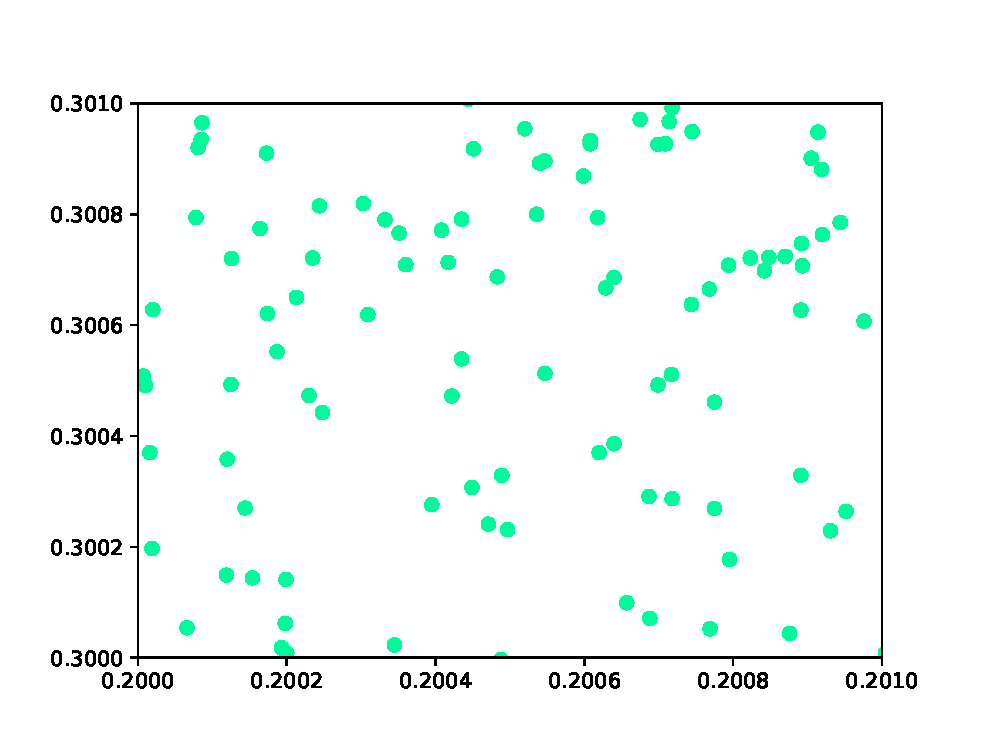
\includegraphics[width=1.2\textwidth]{figures/builtin_zoomed.eps}
        \caption{c++ rand() zoomed}
    \end{minipage}
\end{figure}
\begin{figure}[h]
    \centering
    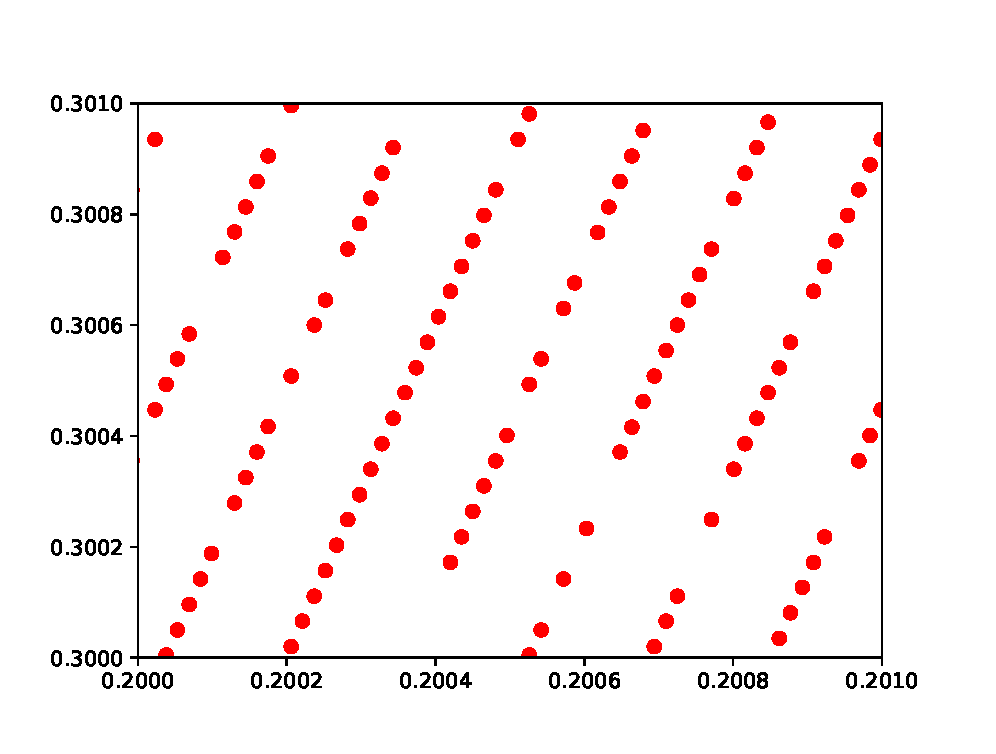
\includegraphics[width=0.6\textwidth]{figures/randu_zoomed.eps}
    \caption{RANDU zoomed}
\end{figure}

\newpage
\section*{Exercise 2}

\begin{figure}[h]
    \centering
    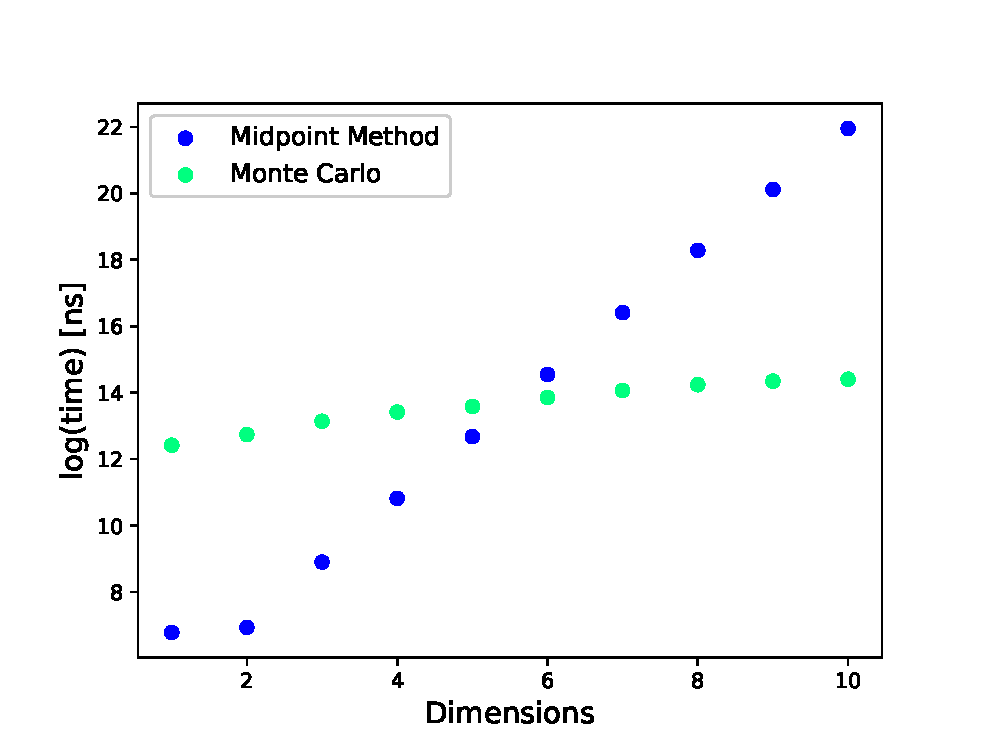
\includegraphics[scale=0.75]{figures/time.eps}
    \caption{Runtime as a function of the number of dimensions}
\end{figure}
\begin{figure}[h!]
    \centering
    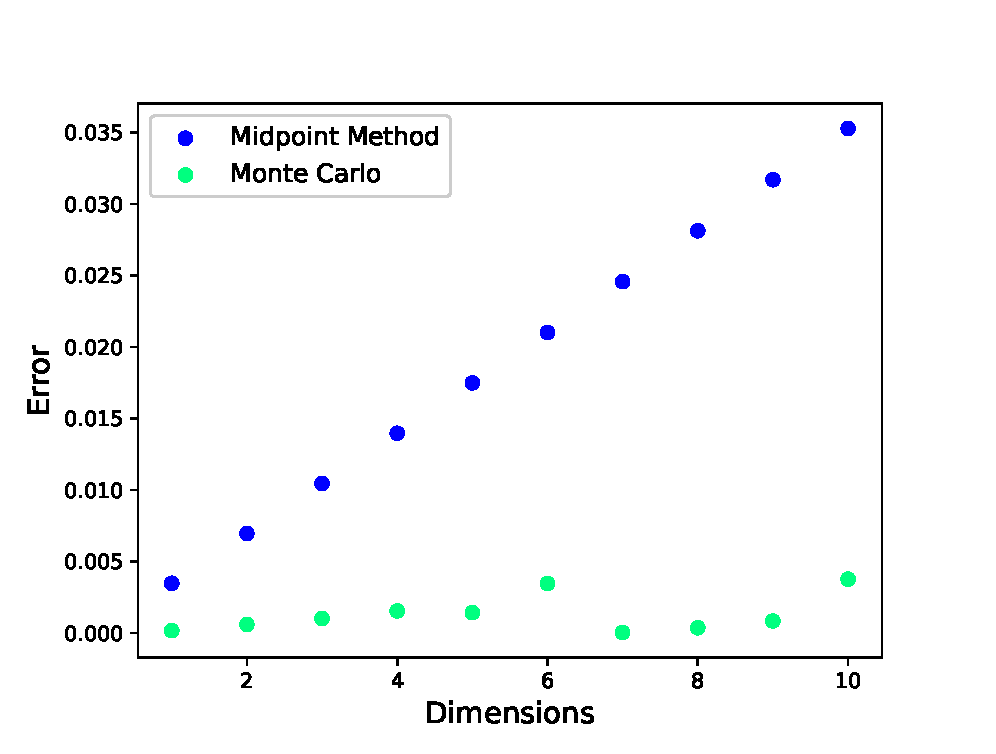
\includegraphics[scale=0.75]{figures/error.eps}
    \caption{Error as a function of the number of dimensions}
\end{figure}

\newpage
\section*{Exercise 3}

\begin{figure}[h]
    \centering
    \begin{minipage}{0.47\textwidth}
        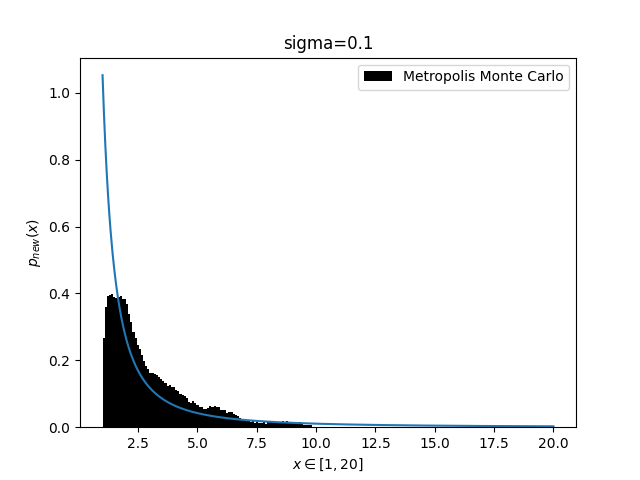
\includegraphics[width=1.2\textwidth]{figures/ex3_sigma01.png}
        \caption{$\sigma = 0.01$}
    \end{minipage}
    \hfill
    \begin{minipage}{0.47\textwidth}
        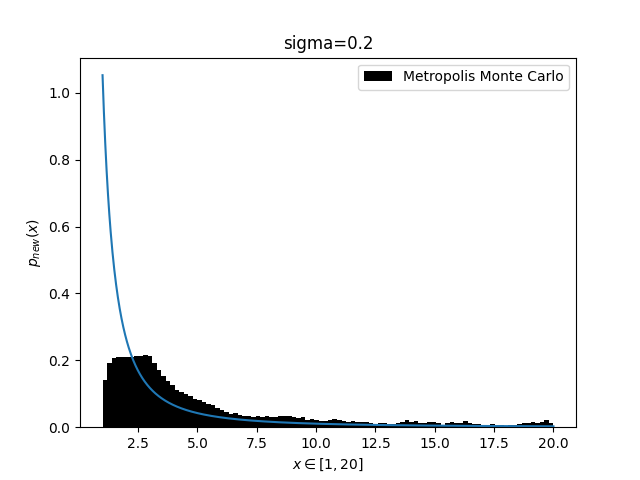
\includegraphics[width=1.2\textwidth]{figures/ex3_sigma02.png}
        \caption{$\sigma = 0.02$}
    \end{minipage}
\end{figure}
\begin{figure}[h]
    \centering
    \begin{minipage}{0.47\textwidth}
        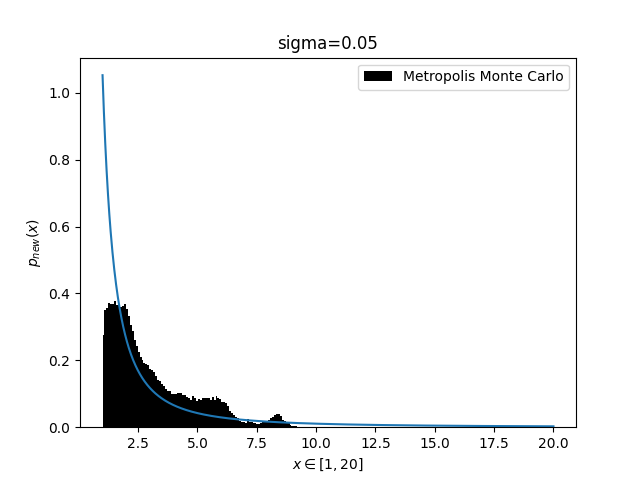
\includegraphics[width=1.2\textwidth]{figures/ex3_sigma005.png}
        \caption{$\sigma = 0.05$}
    \end{minipage}
    \hfill
    \begin{minipage}{0.47\textwidth}
        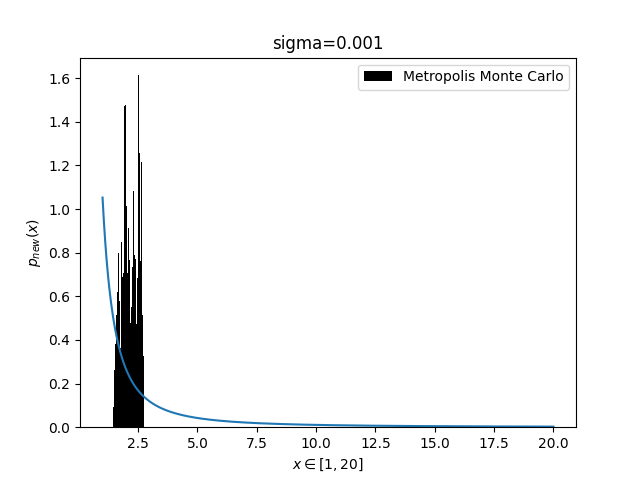
\includegraphics[width=1.2\textwidth]{figures/ex3_sigma0001.png}
        \caption{$\sigma = 0.001$}
    \end{minipage}
\end{figure}
\end{document}